\begin{surferPage}[مثمن شموتوف]{مثمن شموتوف}
     ميزة ملفتة للنظر في مثمن شموتوف $\text{Chm}_{d}, \ d=8,$ وهي تناظره.
     هذا يمكن رؤيته أيضاً من خلال فحص المعادلة:
    \[\text{Chm}_{d}\colon T_d(x) + T_d(y) + T_d(z) + 1 = 0,\]
    حيث $T_d$ هو ما نسميه متعدد حدود شيبيشيف (الصورة على ).
     على يمكن رؤية المنحنى  $T_8(x)+T_8(y)=0$:

     \begin{center}
      \begin{tabular}{c@{\quad}c}
        \begin{tabular}{c}
          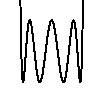
\includegraphics[height=1.75cm]{Tcheb_008.pdf}
        \end{tabular}
        &
        \begin{tabular}{c}
          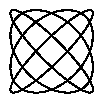
\includegraphics[height=1.75cm]{Tcheb_2d_008.pdf}
        \end{tabular}
      \end{tabular}
    \end{center}
    \vspace{-0.3cm}
    الإنتقال من هذه الصور إلى شكل المنحنى في الصورة التفاعلية مباشر نوعاً ما.


 هذه المعادلات نتجت عن أعمال شموتوف
 \textenglish{(S.V.\ Chmutov)}
  في أوائل الثمانينيات.
   ولقد أوجدت آنذاك الرقم القياسي العالمي $\mu(d)$ للعدد الأقصى للمتفردات لمعظم الدرجات $d$.
    في التسعينيات، حطم شموتوف رقمه القياسي وفي العام 2005، لائم كل من بريسك
     \textenglish{(S.~Breske)} ولابس
     \textenglish{(O.~Labs)}
      وفان ستراتن
     \textenglish{(D.~van~Straten)}
      هذا البناء لمنح منحنيات حقيقية لها متفردات حقيقية فقط.
\end{surferPage}
